\section{Related Work}
\label{sec:related work}

\begin{figure*}[t]
    \centering
    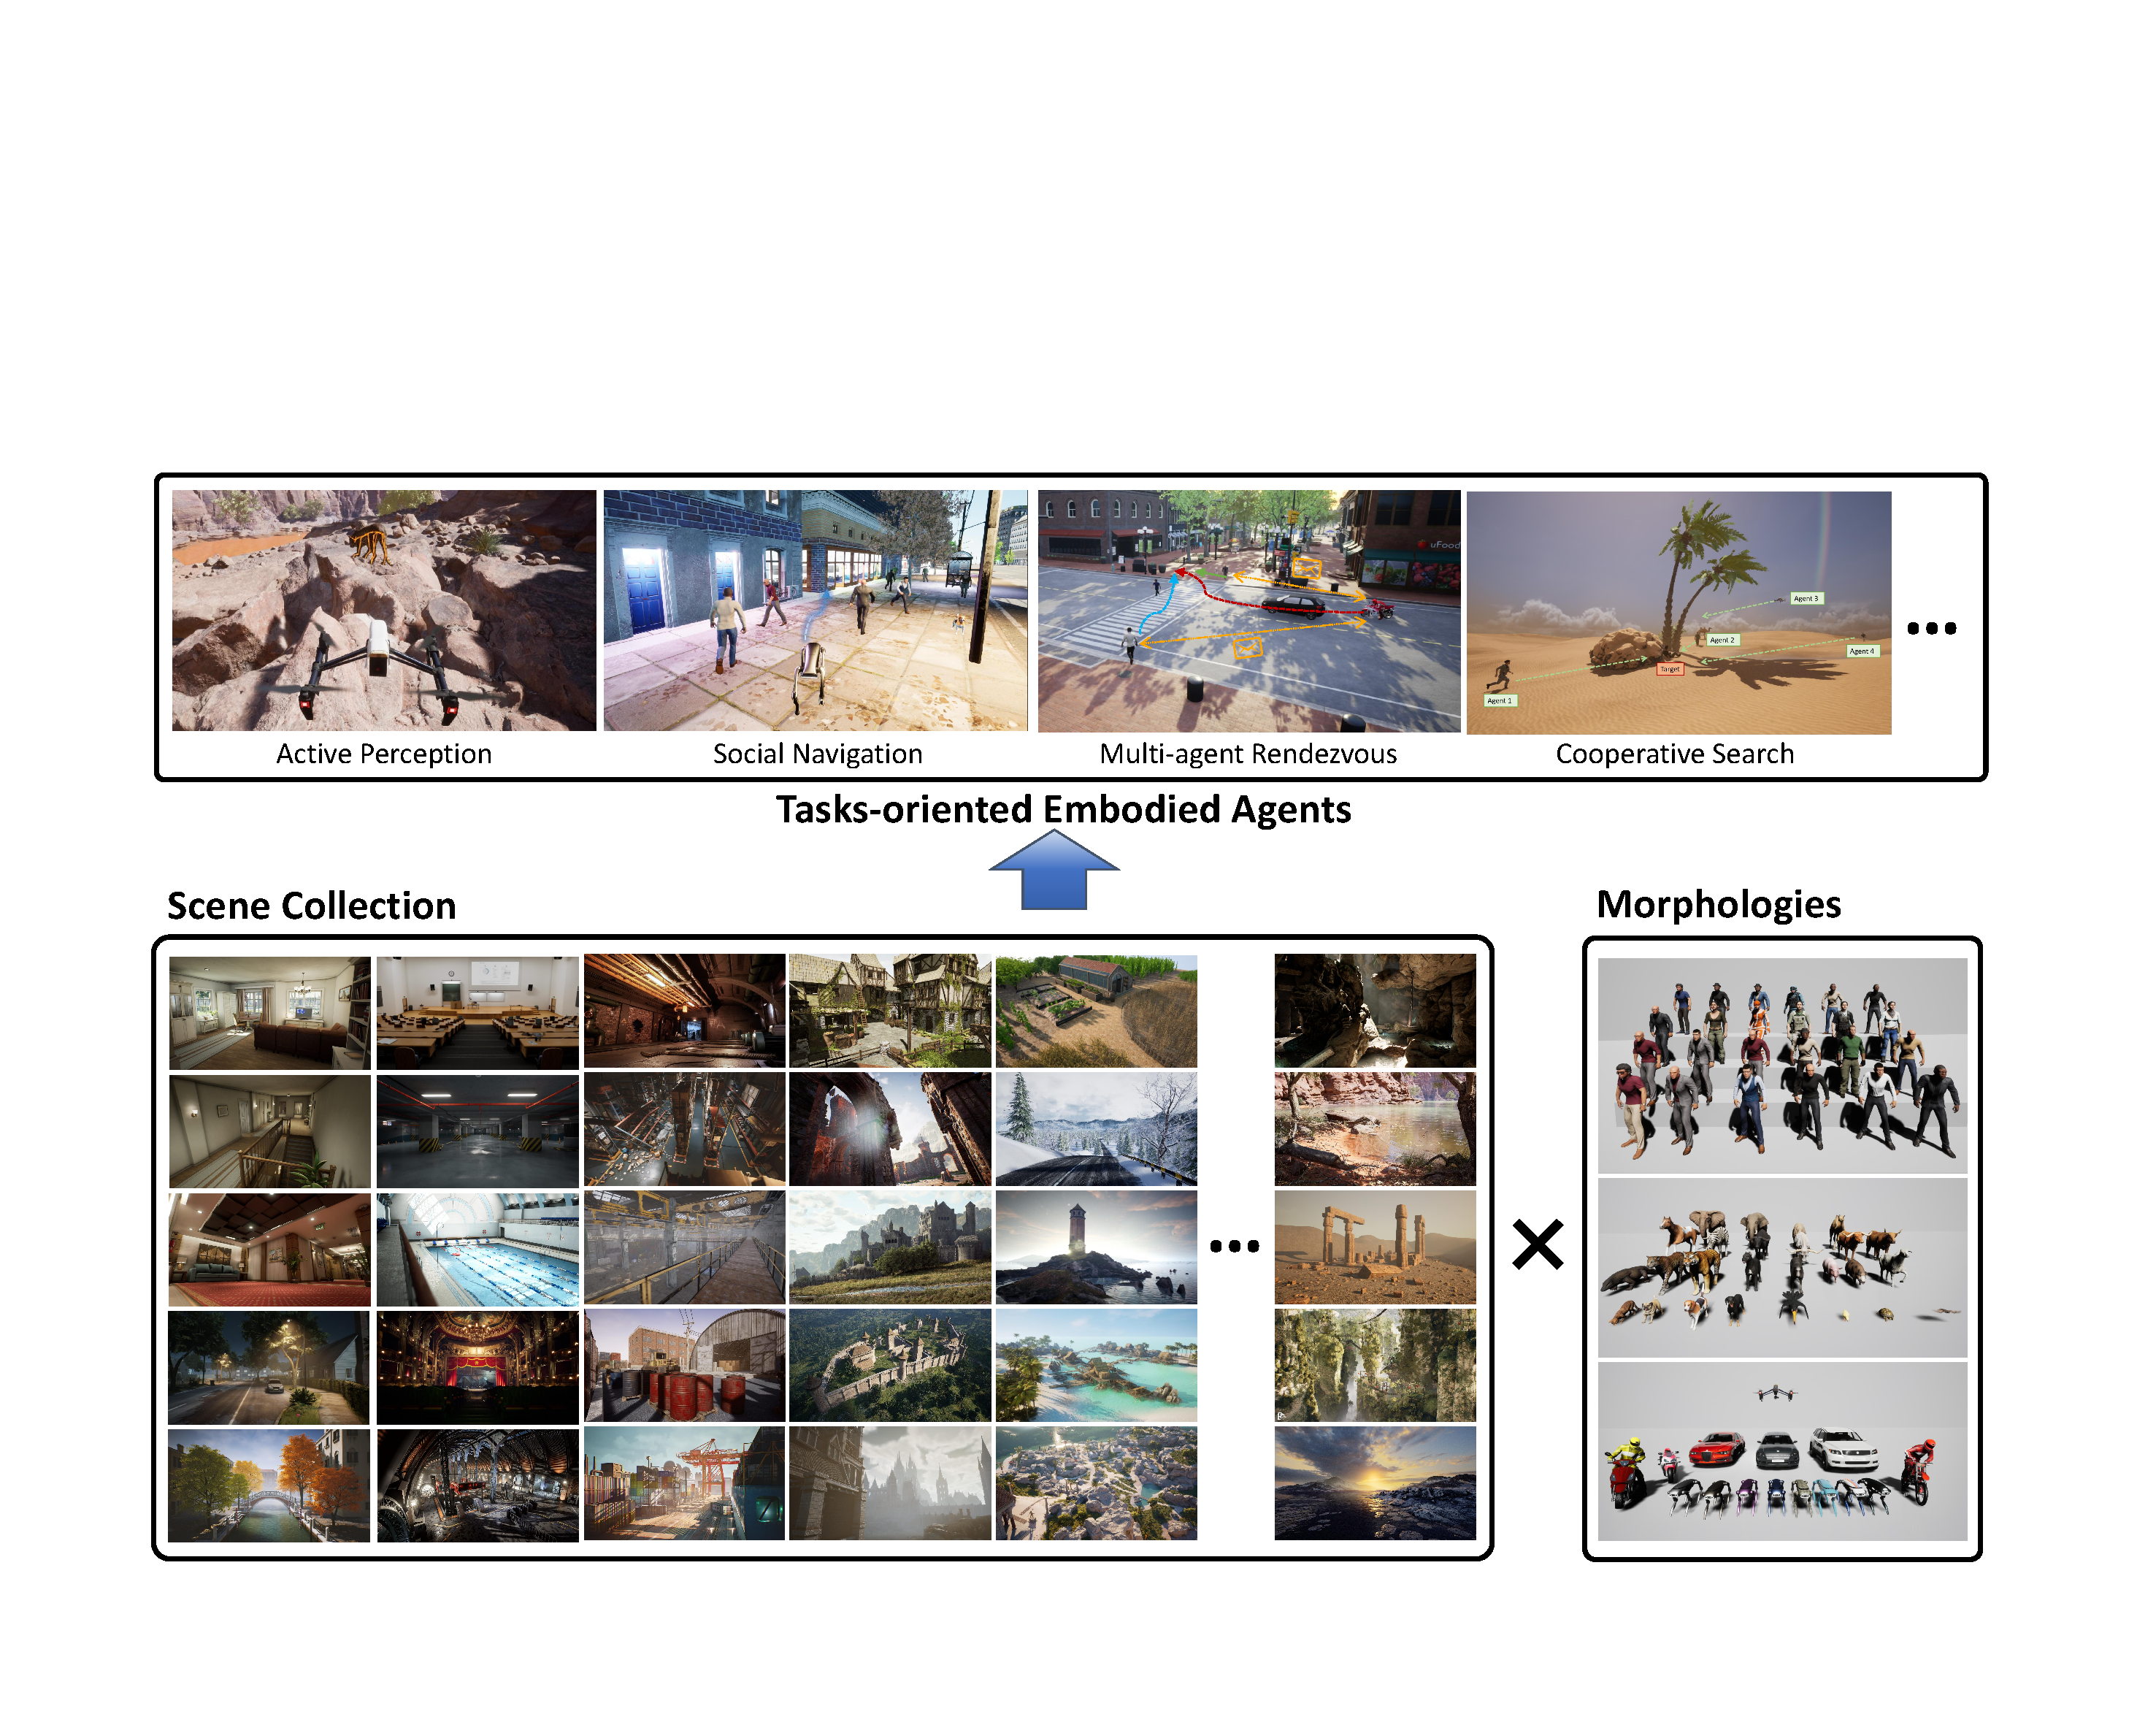
\includegraphics[width=1\linewidth]{figure/overview.pdf}\vspace{-2mm}
    \caption{Overview of the proposed~\name.}
    \label{fig:overview}
\end{figure*}

% \textbf{Video Super-Resolution.}
\paragraph{Video Super-Resolution.} 
Traditional VSR methods can be roughly divided into two categories: recurrent-based \cite{haris2019recurrent, huang2017video, liang2022recurrent, sajjadi2018frame, shi2022rethinking} and sliding-window-based \cite{caballero2017real,liang2024vrt,li2020mucan,xu2021temporal,yi2019progressive} methods. 
Recurrent-based methods process LR video frame by frame using recurrent neural networks \cite{mikolov2010recurrent}. In contrast, sliding-window-based methods divide a video sequence into segments, using each as input to super-resolve the video. 
However, both approaches suffer from degradation mismatch, leading to significant performance drops in real-world applications.
Recently, there has been a growing focus on real-world VSR, targeting complex, unknown degradations. RealBasicVSR \cite{chan2022investigating}, an extension of BasicVSR \cite{chan2021basicvsr}, introduces a pre-cleaning module to mitigate artifacts. 
RealViformer \cite{zhang2024realviformer} discovers that channel attention is less sensitive to artifacts and uses squeeze-excite mechanisms and covariance-based rescaling to address these challenges further. While GAN-based and image diffusion models have made substantial progress, they still face issues such as \textit{over-smoothing details and temporal inconsistency}.

\vspace{-1em}
\paragraph{Text-to-Video Diffusion Model.} 
% \noindent
% \textbf{Text-to-Video Diffusion Model.}
Large-scale pre-trained text-to-video (T2V) diffusion models have garnered significant attention, particularly with the impressive results from Sora \cite{videoworldsimulators2024,sora}. 
Numerous T2V models have since emerged, generally divided into: U-Net-based methods \cite{blattmann2023align, blattmann2023stable, ho2022imagen, singer2022make} and DiT-based methods \cite{yang2024cogvideox, bao2024vidu, polyak2024movie, chen2024gentron}. 
I2VGen-XL \cite{zhang2023i2vgen}, a U-Net-based method, employs a two-stage approach: first generating semantically and content-consistent LR videos, then using these as conditions to produce HR outputs.
CogvideoX \cite{yang2024cogvideox}, built on DiT \cite{peebles2023scalable}, introduces an adaptive LayerNorm to enhance text-video alignment and employs 3D attention to better integrate spatio-temporal information.
Both models %, regardless of architecture, 
have large model capacities and are trained on large-scale datasets, enabling them to capture robust spatio-temporal priors. 
In this work, we propose~\name~to \textit{fully leverage T2V model prior for real-world VSR}.

\vspace{-1em}
\paragraph{Diffusion Prior for Super-Resolution.}
% \noindent
% \textbf{Diffusion Prior for Super-Resolution.}
Several works \cite{wang2024exploiting, lin2023diffbir, yang2023pixel, wu2024seesr, zhao2024wavelet} have leveraged generative diffusion priors for image and video super-resolution. 
StableSR \cite{wang2024exploiting} adds a time-aware encoder and feature warping module to the SD model. DiffBIR \cite{lin2023diffbir} integrates restoration and generative modules via ControlNet, while PASD \cite{yang2023pixel} and SeeSR \cite{wu2024seesr} embed semantic information in U-Net to guide diffusion. These methods balance fidelity and perceptual quality, achieving high-resolution image details.
Methods like Upscale-A-Video \cite{zhou2024upscale}, MGLD-VSR \cite{yang2023mgldvsr}, Inflating with Diffusion \cite{yuan2024inflation}, and SATeCo \cite{chen2024learning} have adapted text-to-image diffusion priors~\cite{rombach2022high,ho2022imagen} for VSR by adding temporal layers. However, rooted in text-to-image models, they often struggle with temporal consistency. 
More recently, VEnhancer\cite{he2024venhancer} and LaVie-SR\cite{wang2023lavie} have incorporated T2V models to super-resolve AI-generated videos but struggle with complex degradations in practical environments. 
In contrast, we are the \textit{first} to integrate powerful T2V diffusion priors for real-world VSR, introducing the LIEM module to address spatial artifacts and DF loss to enhance fidelity.